\section{Thermodynamics and Cosmological Entropy}
\label{ch:thermo_entropy}

\subsection{Introduction to Hyper-Electronic Entropy}
In the framework of Excited-State Cosmology, the observable universe is treated as the internal manifold of an excited hyper-electron. The thermodynamics of this cosmological spacetime can be understood by examining the scaling behavior of its boundary surfaces, conceptually analogous to black hole event horizons. The connection between macroscopic cosmological parameters and microscopic hyper-electronic degrees of freedom is established via holographic scaling laws and the generalized first law of thermodynamics. \cite{Linde1982, Mather1990, Penzias1965}

\subsection{The First Law of Black Hole Thermodynamics}
To mathematically ground the cosmological entropy, we first review the thermodynamics of black holes, beginning with the standard Einstein-Hilbert action:
\begin{equation}
S_{EH} = \frac{1}{16\pi G} \int d^4x \sqrt{-g} R + S_{\text{matter}} + \text{boundary terms}.
\end{equation}
Consider a stationary black hole spacetime containing a Killing horizon $\mathcal{H}$ generated by a Killing vector field $\chi^a = t^a + \Omega_\mathcal{H} \phi^a$, where $t^a$ is the time-like Killing vector (normalized to $-1$ at infinity), $\phi^a$ is the rotational Killing vector, and $\Omega_\mathcal{H}$ is the angular velocity of the horizon. The surface gravity $\kappa$ is defined geometrically on the horizon by the non-affinity of the geodesic equation for the Killing generators:
\begin{equation}
\chi^b \nabla_b \chi^a = \kappa \chi^a \quad \text{on} \quad \mathcal{H}.
\end{equation}
By evaluating the conserved Noether currents associated with the diffeomorphism invariance of the action, we can relate the variations of the asymptotic charges to properties defined on the horizon. For a variation between two nearby stationary black hole solutions, the change in the ADM mass $M$, angular momentum $J$, and horizon area $A$ are related by the first law of black hole mechanics:
\begin{equation}
\delta M = \frac{\kappa}{8\pi G} \delta A + \Omega_\mathcal{H} \delta J.
\end{equation}
This classical geometric relation strongly suggests a thermodynamic interpretation, provided one can consistently associate a physical temperature and an entropy with the black hole horizon.

\subsection{Bekenstein-Hawking~\cite{Bekenstein1973, Hawking1975} Entropy}
The thermodynamic analogy is fully realized through quantum field theory in curved spacetime. Hawking's derivation indicates that black holes emit thermal radiation with a temperature exactly proportional to the surface gravity:
\begin{equation}
T_H = \frac{\hbar \kappa}{2\pi k_B c}.
\end{equation}
Substituting this Hawking temperature into the first law of black hole mechanics, and comparing it directly with the standard thermodynamic relation $dE = T dS + \text{work terms}$, we can identify the differential Bekenstein-Hawking entropy:
\begin{equation}
dS_{BH} = \frac{k_B c^3}{4 G \hbar} dA.
\end{equation}
Integrating this relation for a black hole forming from zero initial area yields the celebrated Bekenstein-Hawking formula:
\begin{equation}
S_{BH} = \frac{k_B A}{4 \ell_P^2},
\end{equation}
where $\ell_P = \sqrt{\frac{G\hbar}{c^3}}$ is the fundamental Planck length.

\subsection{The Internal Entropy Matrix of the Excited Hyper-Electron}
We now apply these foundational principles to the macroscopic state of the universe viewed as the internal manifold of the hyper-electron. In this model, the total entropy is formulated as the trace of a reduced density matrix $\rho_{\text{int}}$, characterizing the quantum entanglement between the internal spatial slices of the universe and the external unobservable bulk space of the hyper-electron.
The entanglement entropy is given by the standard von Neumann entropy formula:
\begin{equation}
S_{\text{int}} = -k_B \text{Tr}(\rho_{\text{int}} \ln \rho_{\text{int}}).
\end{equation}
According to the generalized holographic principle applied to the hyper-electronic boundary, the maximal entropy associated with any causally connected region scales dynamically with the area of the apparent cosmological horizon $A_c = 4\pi R_c^2$, where $R_c$ is the Hubble radius. Thus, the entropy matrix eigenvalues are constrained such that the trace scales as:
\begin{equation}
S_{\text{int}} \simeq \frac{k_B A_c}{4 \ell_P^2} = \frac{\pi k_B R_c^2}{\ell_P^2}.
\end{equation}
This precise scaling law represents the bounding constraint on the thermodynamic phase space of the observable universe, explicitly tying the accelerated expansion of the cosmological manifold to the increasing informational capacity of the hyper-electron's internal state.


\begin{figure}[H]
\centering
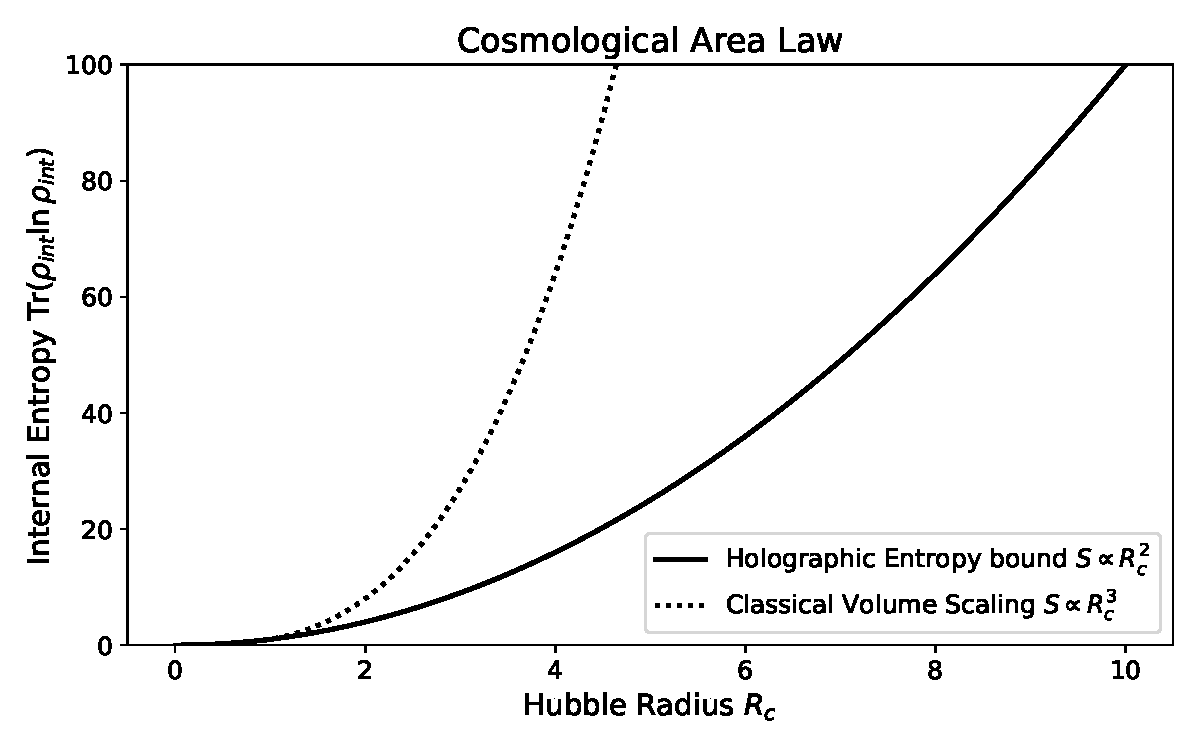
\includegraphics[width=0.85\textwidth]{fig_ch10.pdf}
\caption{Mathematical visualization of the principles derived in Section 10.}
\end{figure}
